\documentclass[a4paper,11pt]{jsarticle}


% 数式
\usepackage{amsmath,amsfonts}
\usepackage{bm}
\usepackage{physics}
% 画像
\usepackage[dvipdfmx]{graphicx}
% ローマ数字
\usepackage{otf}
% 単位
\usepackage{siunitx}
% 表
\usepackage{multirow}
% 化学反応
\usepackage[version=4]{mhchem}


\begin{document}

\title{理論演習}
\author{齋藤駿一}
\date{\today}
\maketitle

\section{概要}
まず,エラー率0のときのモデルを解析的に考察し,栄養濃度$n=1$における成長速度の転移が「トランスクリティカル分岐」によるものと分かった.

次に,エラー率が成分濃度に依存するモデルを考えた.
ここでは,最大エラー率$\delta$の値を何通りかとって,それぞれについて栄養濃度$n$と成長速度の関係を調べた.
その結果,$\delta$が増すと,栄養濃度の閾値(成長できるか否かの境目)が$\delta$と同じくらいのオーダーで増加することが確認できた.
ただし,エラー率が栄養分子の濃度に依存する場合,$\delta$が大きいとき例外的にこの閾値が急増した.

最後に,姫岡先生のモデルと対応づけるため,栄養環境を途中で変えるシミュレーションを行ったが,「復活できずに死んでしまう」挙動などが再現できなかった.

\section{エラー率0における成長速度の転移とべき減衰についての考察}

最も簡単な反応ネット$[[1,0,0]]$を考察する.
膜分子濃度$x_0$の従う微分方程式は,
\begin{equation}
  \frac{dx_0}{dt} = \epsilon x_0 x_1 - \epsilon_g x_0 - \mu x_0 
\end{equation}
である.
仮定$\mu = g\epsilon_g x_0$より,これは
\begin{equation}
  \frac{dx_0}{dt} = \epsilon x_0 x_1 - \epsilon_g x_0 - g \epsilon_g x^2_0 = \epsilon_g x_0 (\frac{\epsilon}{\epsilon_g} x_1 - 1 - g x_0)
\end{equation}
と書き換えられる.
ここで,内部栄養濃度は外部栄養濃度と等しい($x_1 = n$)と近似すると,これは1変数のロジスティック方程式
\begin{equation}
  \frac{dx_0}{dt} = \epsilon_g x_0 (\frac{\epsilon}{\epsilon_g} n - 1 - g x_0) \label{logistic}
\end{equation}
となる.
この方程式の定常解のうち安定なものは,栄養濃度$n$によって
\begin{equation}
  \begin{cases}
    \frac{\epsilon}{\epsilon_g} n - 1 > 0 \text{のとき} & x_0 = \frac{1}{g} \left( \frac{\epsilon}{\epsilon_g} n - 1 \right) \\
    \frac{\epsilon}{\epsilon_g} n - 1 < 0 \text{のとき} & x_0 = 0
  \end{cases}
\end{equation}
と分岐(トランスクリティカル分岐)する.
したがって,成長速度が正,つまり$x_0 > 0$であるには,栄養濃度は$n > n^* = \epsilon_g/\epsilon$が満たされている必要がある.
前回はとくに$\epsilon = \epsilon_g = 1$としていたので,この閾値が$n^*=1$となっていた.
このことは,ロジスティック方程式\eqref{logistic}において,膜分子の生成($n$に依存する)と消費($n$に依存しない)のバランスを考えることで直観的に理解できる.

また,$n \neq n^*$のとき,ロジスティック方程式\eqref{logistic}の厳密解として
\begin{equation}
  x_0(t) = \frac{a}{g + Ce^{-a\epsilon_g t}} \qquad (C\text{は積分定数})
\end{equation}
が得られる.ただし,
\begin{equation}
  a = \frac{\epsilon}{\epsilon_g} n - 1 = \frac{n}{n^*} - 1
\end{equation}
とおいた.
ここで,$\lvert a\rvert \ll 1$とすると,指数関数をテイラー展開することにより,
\begin{align}
  \frac{1}{x_0(t)} &= \frac{g + Ce^{-a\epsilon_g t}}{a} \notag\\
  &\approx \frac{g + C - Ca\epsilon_g t + \mathcal{O}((at)^2)}{a} \notag\\
  &= \frac{1}{x_0(0)} - C\epsilon_g t + \mathcal{O}(at^2)
\end{align}
となって,$x_0(t)$は$at^2$が小さい間は$t^{-1}$でべき減衰することが分かる.
さらに時間が経つと,$at$の高次の項が無視できなくなり,$t^{-n} \,(n=2,3,\cdots)$のべき減衰が次々に現れると考えられる.

また,反応ネットを$[[1,0,0],[0,1,0]]$に変更しても,最初の微分方程式に$-\epsilon x^2_0$の項が加わることで$g \to g + \epsilon/\epsilon_g$となるだけで,他はまったく同じ議論である.
一般に,反応ネットが変わっても,$x_0$または$x^2_0$の項が付け加わるだけならば,同じ議論が成り立つ\footnote{ただし,閾値$n^*$が負になって任意の栄養濃度で成長できるようになる可能性はある.また,定数項が付け加わると転移が起こらなくなる.}.

\section{最大エラー率$\delta$,栄養濃度$n$と成長速度の関係}

前回,エラー率$e$を成分濃度$x=x_0,x_1$に依存させて
\begin{equation}
  e = \frac{\delta}{1+x}
\end{equation}
とおき,$x=x_0$の場合と$x=x_1$の場合で最終的な成長速度に差が生まれる栄養濃度は
\begin{equation}
  n = 1 + \delta
\end{equation}
程度であることが分かった.
今回は,より具体的に,いくつかの$\delta, n$に対して,$t=10^5$時点での成長速度をプロットした.
その結果,$\delta=0,\,0.001\,0.01,\,0.1,\,0.7,\,1$に対してそれぞれ図\ref{fig:errslp0_ng},図\ref{fig:errslp0001_ng},図\ref{fig:errslp001_ng},図\ref{fig:errslp01_ng},図\ref{fig:errslp07_ng},図\ref{fig:errslp1_ng}が得られた.
これらより,$\delta$が大きくなるにつれて,栄養濃度の閾値が高くなることが分かった.
また,上の関係式は,今回調べた$\delta=10^{-3} - 1$の範囲では,おおよそ正しいことが確認できた.

\begin{figure}[htbp]
  \centering
  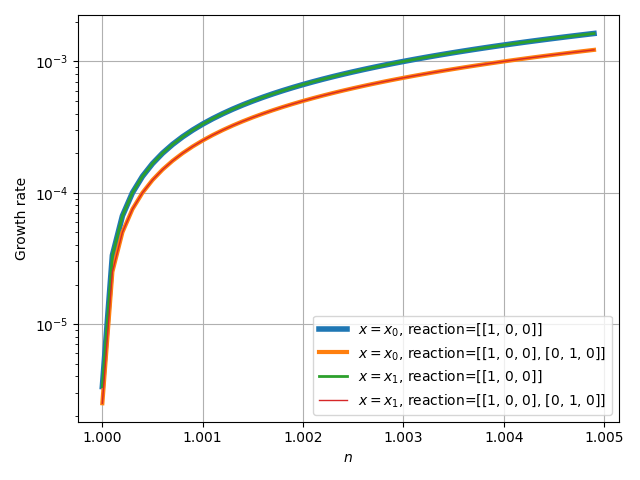
\includegraphics[width=10cm]{waste_errslp0_s01_ng_focus.png}
  \caption{$t=10^5$における栄養濃度と成長速度の関係($\delta=0$).ただし,$n=1$での成長速度は減衰の途中であることを確認した(図は省略するが,$t=10^6$でプロットし直すと$1/10$程度に減っていた.これは先述したべき減衰である.).}
  \label{fig:errslp0_ng}
\end{figure}

\begin{figure}[htbp]
  \centering
  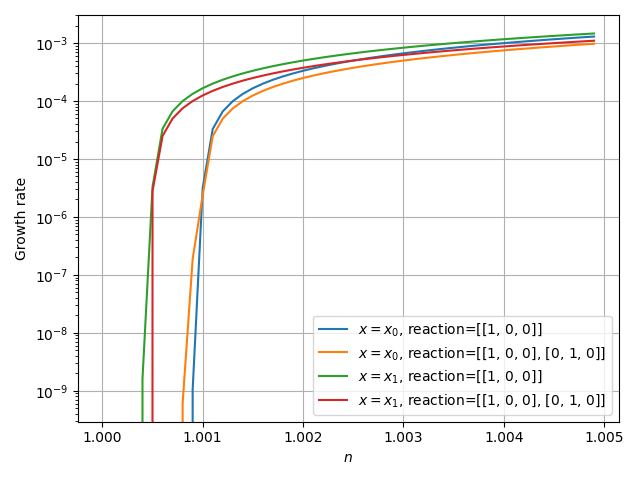
\includegraphics[width=10cm]{waste_errslp0001_s01_ng_focus.png}
  \caption{$t=10^5$における栄養濃度と成長速度の関係($\delta=0.001$).}
  \label{fig:errslp0001_ng}
\end{figure}

\begin{figure}[htbp]
  \centering
  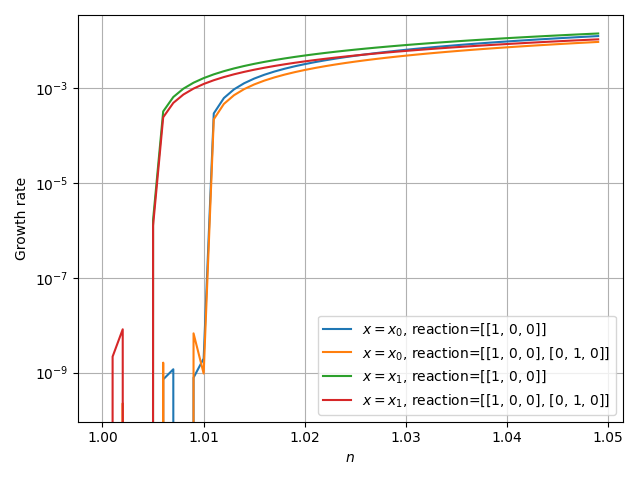
\includegraphics[width=10cm]{waste_errslp001_s01_ng_focus.png}
  \caption{$t=10^5$における栄養濃度と成長速度の関係($\delta=0.01$).}
  \label{fig:errslp001_ng}
\end{figure}

\begin{figure}[htbp]
  \centering
  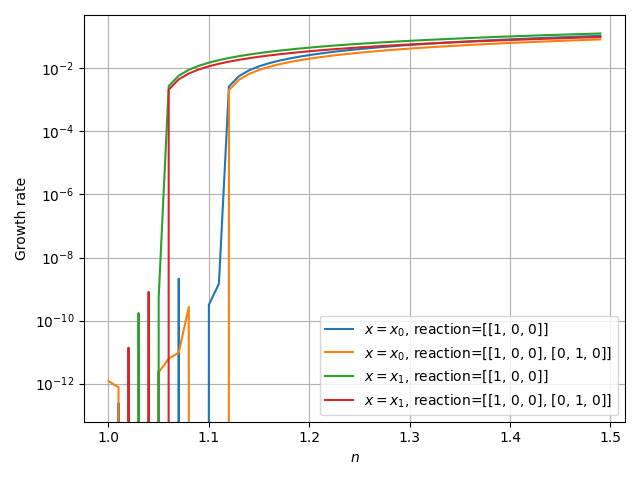
\includegraphics[width=10cm]{waste_errslp01_s01_ng_focus.png}
  \caption{$t=10^5$における栄養濃度と成長速度の関係($\delta=0.1$).}
  \label{fig:errslp01_ng}
\end{figure}

\begin{figure}[htbp]
  \centering
  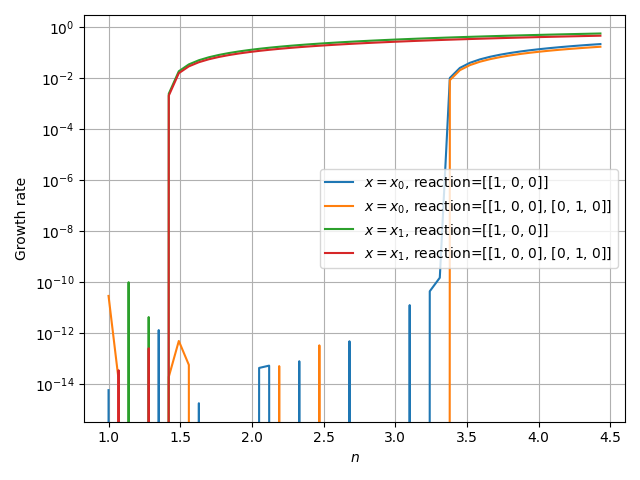
\includegraphics[width=10cm]{waste_errslp07_s01_ng_focus.png}
  \caption{$t=10^5$における栄養濃度と成長速度の関係($\delta=0.7$).}
  \label{fig:errslp07_ng}
\end{figure}

\begin{figure}[htbp]
  \centering
  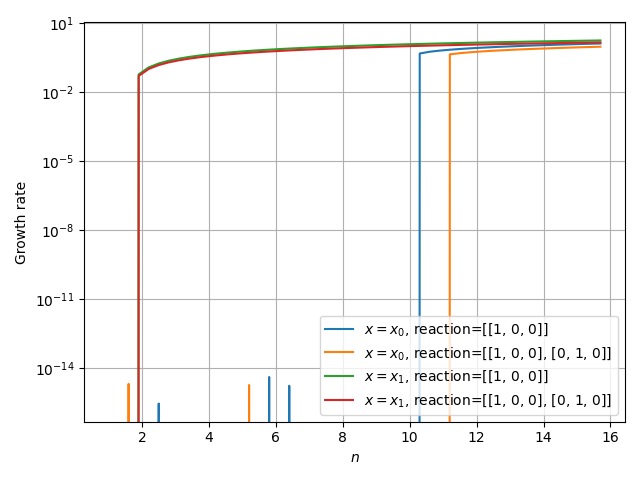
\includegraphics[width=10cm]{waste_errslp1_s01_ng_focus.png}
  \caption{$t=10^5$における栄養濃度と成長速度の関係($\delta=1$).}
  \label{fig:errslp1_ng}
\end{figure}

\section{ラグタイムの確認}
最後に,ここで作成したモデルが姫岡先生のモデルと対応することを確認するために,栄養濃度$n$を途中で変える実験を行った.

まず,反応ネットを$[[1,0,0],[0,1,0]]$,エラー率0として,時間$T_{\mathrm{stv}}=10^2$の間$n=n_1=0.9<1$の飢餓状態において濃度を時間発展させた後,成長できる環境$n=n_2=2$に戻すと,次のような図が得られた.
ゴミ分子がないので,当然ながらラグタイムは見られなかった.

\begin{figure}[htbp]
  \centering
  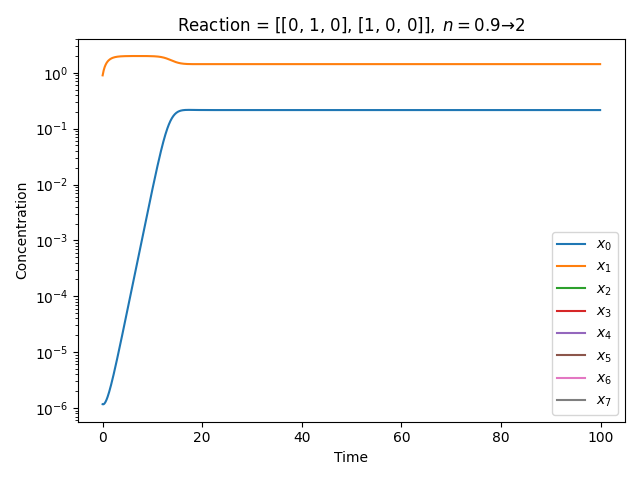
\includegraphics[width=10cm]{waste_err0_lag_T2_n09to2.png}
  \caption{エラー率0で見られた典型的な挙動($x_0$は膜分子濃度,$x_1$は内部栄養濃度.).エラーが起きないため,ゴミ分子$x_2,x_3$や複合体$x_4,x_5,x_6,x_7$の濃度は常にゼロである.}
  \label{fig:err0_lag}
\end{figure}

そこで,エラー率を成分濃度に依存させて,パラメータ$\delta,n_1,n_2,T_{\mathrm{stv}}$を変えたが,今のところラグタイムを確認できていない(図\ref{fig:err1_lag}).

\begin{figure}[htbp]
  \centering
  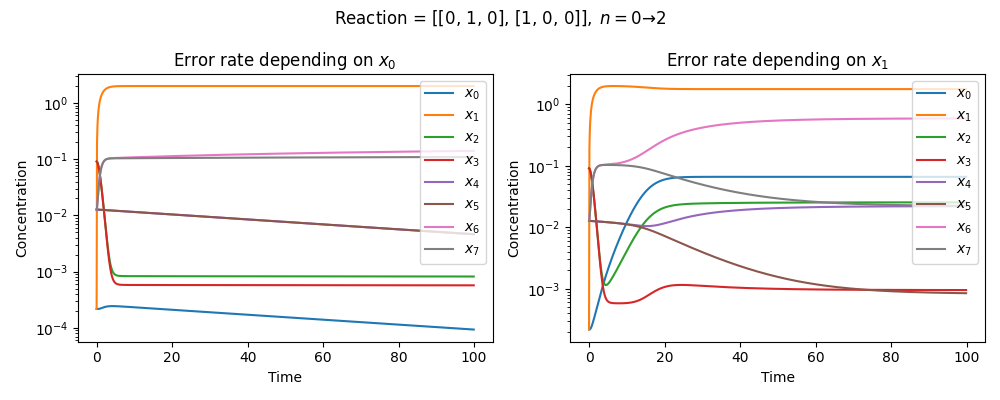
\includegraphics[width=\columnwidth]{waste_errslp1_lag_T2_n0to2.png}
  \caption{反応ネット$[[1,0,0],[0,1,0]]$,最大エラー率$\delta=1$で,栄養濃度を$n=0$として飢餓時間$T_{\mathrm{stv}}=10^2$の間放置してから,$n=2$に変えた後の成分濃度の時間発展($x_0$は膜分子濃度,$x_1$は内部栄養濃度,$x_2,x_3$はゴミ分子濃度,$x_4,x_5,x_6,x_7$は複合体濃度.初期濃度は$x_0=x_1=1$,他はゼロ.).}
  \label{fig:err1_lag}
\end{figure}

\newpage
\section{レポート用のメモ(ここで扱ったモデルの性質まとめ)}

\begin{enumerate}
  \item エラー率0,成分数2で成長速度の転移が見られる.(栄養濃度と成長速度の関係から成分濃度のべき減衰まで,解析的に説明がつく.)
  \item ゴミ分子,複合体を導入したが,直感に反するような現象が見つからない.(成長のためにはエラー率0よりも良い栄養環境が必要になる.エラー率は,膜成分よりも栄養成分に依存させた方が成長しやすい.)
  \item ラグタイムが今のところ見つからない.(姫岡先生のモデルと対応していない?)
\end{enumerate}
\end{document}